\section{Building a repository} \label{BuildRep}
We have already seen an overview of what has been created, but we will now go into details about how we got here. As already discussed in the actor model section '\nameref{AMRelation}' our driving force for the project has been to examine four cases relating the actor model to the CLS, namely:
\begin{enumerate}
	\item Synthesizing objects with timers. This was primarily aimed to be accomplished in the player object through the use of different abilities.
	\item Disposing timers. As both the monsters and the boss has recurring timers and they both can be killed, it is important that we ensure their timers are disposed correctly. If not we might end up with 'invisible' enemies hitting players throughout their adventure.
	\item Synthesizing an object which spawns actors. This is accomplished in the boss with its baseline ability to spawn small monsters in the room with it.
	\item Handling a list of arguments in our meta language. We see this in the weather effects in the rooms where a random weather effect from a given list can be chosen and will have an effect on the players each time they change room.
\end{enumerate}
Our overall goal with this project has been to examine if it is possible to synthesize actor code with the use of the CLS and we found that the four cases above would not be comprehensive but we see the first three to be common tasks performed when coding with the actor model, and the last we foresee to be a common way to program with meta languages when using the CLS. We therefore see the four cases as a good indication of whether it is possible synthesize actor code on a larger scale rather than a definitive answer to the CLS being a perfect tool to synthesize actor code.\\

Throughout development we found that the coupling between the oldest objects we coded and the newest grew bigger and bigger. This is a tendency we think is rather common in software development (and perhaps also logically) if developers are not careful about their designs and encapsulation. This might also have been an indication that we should have taken a step back and tried to modularize our code more than we have. The fact that the coupling grew with each addition of features made decomposition harder, and finding meaningful decompositions hard as we might just have wanted to change a few lines of code somewhere. In this rather small project we have managed to work around the coupling, at least to a satisfying extent. However, this might not be the case in bigger projects, and thus our first point to stress is that actors should truly be isolated to allow for good decomposition. To achieve clean repositories we need close to no coupling between objects, and thus good design of programs are essential for decomposition. \todo{Point for conclusion here.}

\subsection{Player} \label{BuildPlayer}
\begin{wrapfigure}{L}{0.55\linewidth}
	\vspace{-10px}
	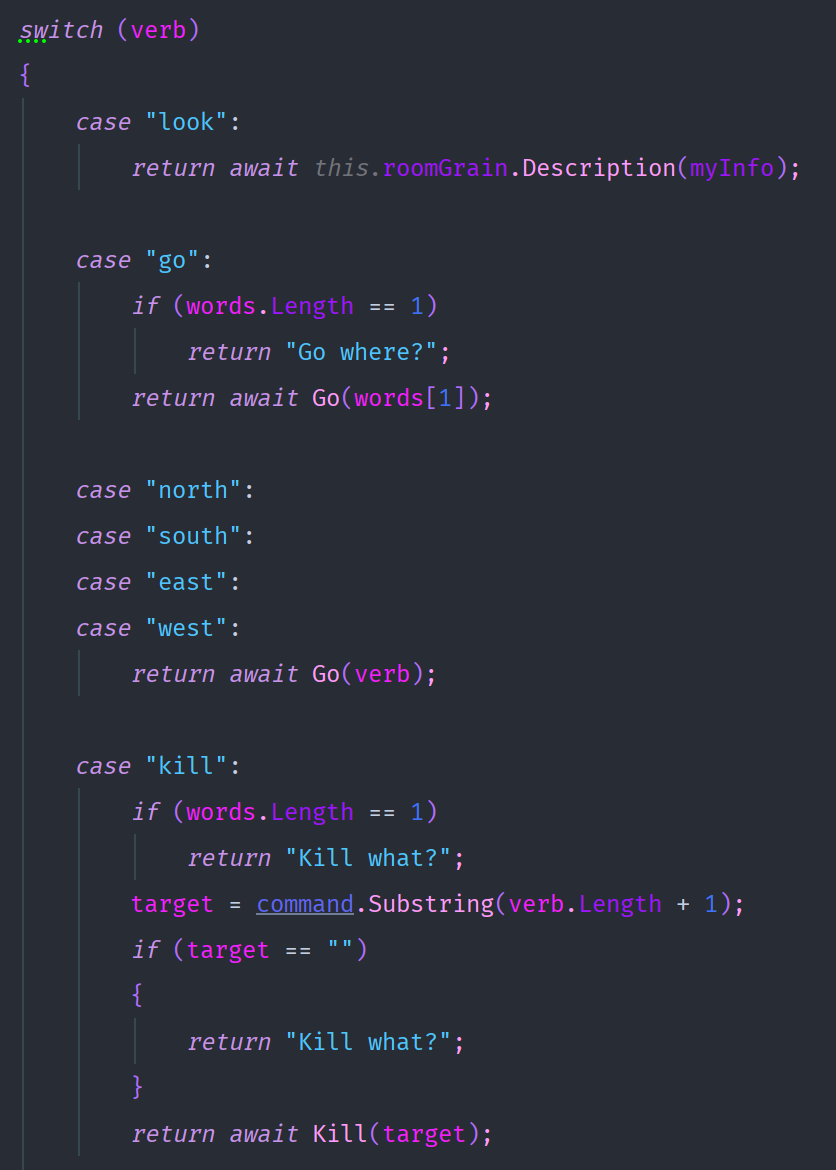
\includegraphics[width=\linewidth]{Materials/Decomposition/switchcases}
	\caption{Part of the switch case in player showing how some actions are implemented.}
\end{wrapfigure}
The player was the first object we implemented and the first we combinated. To understand how we chose to decompose the player we will first look at what makes a player. The player is implemented with a switch case with a case for all the actions the player can take. If we want to move to a new room we could for instance use the command 'go' followed by the direction we want to move. We can semantically look at the switch case as our 'case' or 'cases'.\\
A big part of what makes a player is the abilities it can use. For our implementation we have three variations of what abilities a player can use: fireball, roar or none. As already mentioned \todo{Reference our implementation} does the fireball and roar fulfil two different purposes. The fireball deals damage, and the roar makes the player take less damage. This left us with a choice of either accepting that we would need more information in the form of an extra combinator to ensure that we do not end up with dead code, or to accept the dead code, but making modularization  easier.\\
In our first iteration of the player we wanted to avoid the dead code. This made it hard to modularize the concept of an ability. The fireball simply calls the enemy's take damage function with a higher damage value than the player's standard attack. On the other hand, the roar ability sets a flag in the player which ensures when an enemy attacks, another branch is taken in the player's \textit{TakeDamage} method. The method can be seen in \autoref{PlayerTakeDamage}. To avoid dead code we added more semantic information when we created our repository. Two combinators which provided code with semantic type \textit{'damageTaken'} were thus made. The first having an implementation which did not use the field \textit{'roarActive'} and only had a single line for taking damage, and the second having the full if statement as seen in \autoref{PlayerTakeDamage}.

\begin{figure}[H]
	\centering
	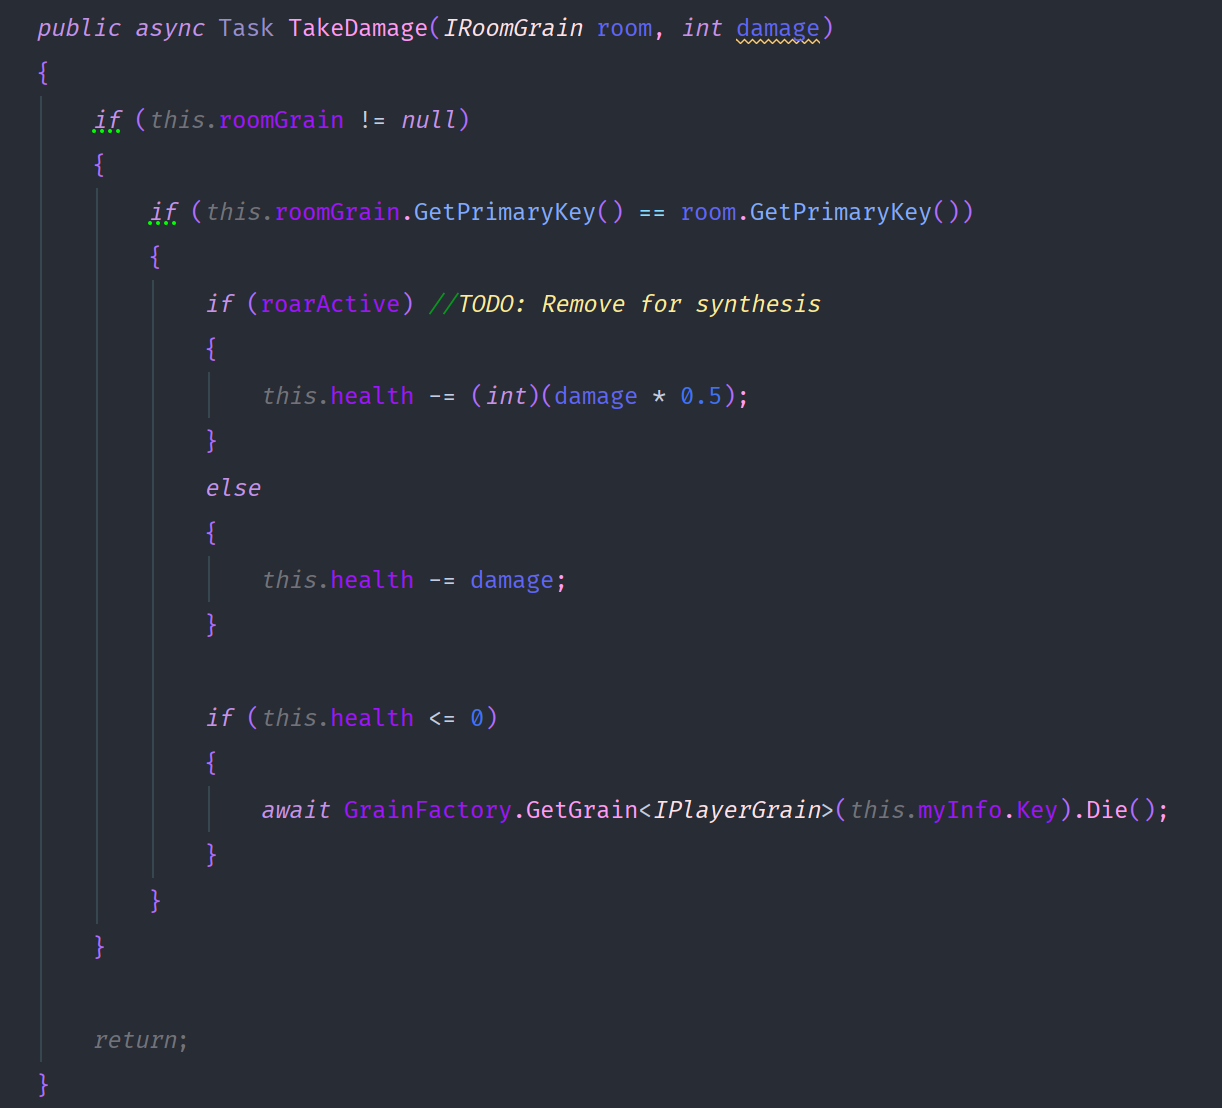
\includegraphics[width=0.8\linewidth]{Materials/Decomposition/TakeDamage}
	\caption{The player's TakeDamage method. Note the if case for when the roar ability is active. Having this if statement means we either need more combinators to describe the synthesis we want, or we have to accept we have dead code. }
	\label{PlayerTakeDamage}
\end{figure}
One can now ask, why is it important not to have dead code? Having dead code means we have fragments of other variations in the code. This means we suddenly have code that does not necessarily makes sense in the current context. A consequence of this could be that we try to access an object that does not exist, making the whole program crash. In general we risk unexpected behaviour which in worst case leads to a crash. This can however be mitigated through thorough testing, showing that it is at least not immediately apparent how the code will show unexpected behaviour based on the dead code \todo{Do we agree that's how testing works?}.\\
On the concrete example of \textit{'TakeDamage'} we see that \textit{'roarActive'} has to be true for the player to take half damage. Designing the player such that the only time this field is set to true is in the roar ability, it would be rather safe to leave the if statement in, as it should not ever be reachable this way. This also made the argument for choosing to leave the dead code and simplify modularization of abilities. However, as we ran out of development time we have not been able to refactor the old code. It could however easily be refactored such that we used dependency injection to give the player an ability which would be its own object with a \textit{'useAbility'} method allowing the player object to call this whenever it needs. The fireball implementation would then call the enemy's \textit{'kill'} method with a high damage value, and the roar implementation would set \textit{'roarActive'} in the player.\\ \todo{Stating we are not going to change player implementation.}
One could argue that in traditional software development it would not be possible to leave dead code in the implementation as we argue in the above that we can, and thus the above is not truly a modularization of the player. To that it could be argued that creating the combinators using the semantic type \textit{'damageTaken} opens up for possible extensions. If there had to be made combinators for how the player takes damage, we have effectively unified what caused the original problem, that an ability both could deal damage and affect how the player takes damage. The only problem here is how we carry this information and rather poor scaleability. Before getting into that we will summarize on the semantics that makes a player.\\
In our concrete implementation the semantics of a player is split in three parts, its actions, its ability and how it takes damage. As already discussed, we have the switch case of actions a player can take and to be able to perform an ability a case needs to be added here. Semantically we can call this a \textit{'case'}. Not surprisingly we can relate the players ability to the semantic type \textit{'ability'}. Lastly we will refer to how the player takes damage with the semantic type \textit{'damageTaken'}. We can thus describe a player as: \textit{string $\cap$ case, string $\cap$ ability, string $\cap$ damageTaken $\to$ MyResult $\cap$ player}. \todo{Unsure if this is a way to long explanation just to reach this rather anticlimactic point?}

\begin{figure}[H]
	\centering
	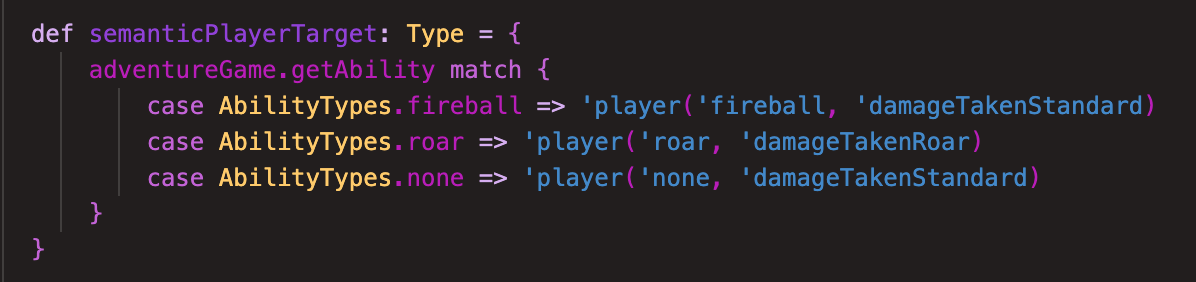
\includegraphics[width=0.9\linewidth]{Materials/Decomposition/SemanticTargetPlayer}
	\caption{The function determining what semantic types in the player we are looking for in our variations.}
	\label{SemanticTargetPlayer}
\end{figure}
So why did we say this approach would scale poorly? This is due to how we carry the information about which variation we want to synthesize. To this we are using \textit{kinding} which allows us to specific about our semantic types. As seen in \autoref{SemanticTargetPlayer} we can for instance have a semantic type \textit{'player('fireball, 'standardDamageTaken}. Here the types \textit{fireball} and \textit{damageTakenStandard} are kindings of respectively \textit{ability} and \textit{damageTaken}. The semantic types (of the same names) can now take these kindings and that way we create the variation we want. For the player the semantic type \textit{'case'} takes the same kinding as the semantic type \textit{'ability'} and that way we always get the corresponding ability to a case. But as we already have noted a player takes two kindings. This is the reason this approach does not scale. If we for each ability have to create combinators and create kindings to carry information forward it will not be feasible to write out all the possible outcomes when appending to the \textit{'semanticPlayerTarget'} function (seen in \autoref{SemanticTargetPlayer}).\\
We previously discussed how we could avoid using the semantic type \textit{'damageTaken'} and obtain more modularization by accepting dead code. Using this approach we can describe a player as: \textit{string $\cap$ case, string $\cap$ ability $\to$ MyResult $\cap$ player}. This approach would avoid introducing more kindings than \textit{ability} and would thus seem more scaleable. However, tweaking the damage reduction for the player would seem problematic but adding other ways to deal damage and adding abilities with different 'purpose' than dealing damage and reducing it would also seem easily done.\\

The player fulfilled the purpose of being an entity with timers. When synthesising the abilities we also include code for timers for the two possible abilities. We can thus say that we successfully can synthesize actor code which uses timers. However, these timers are very simple. They do not require disposing as the player only seizes to exist when the program is closed. Further, these timers are never recurring, so they only fire when the player asks them to. This essentially means that our only consideration with timers for the player is the abilities cool downs (the time before we can use the ability again, because being able to use the abilities repeatedly would make the player way too strong).  
\subsection{Monster and Boss}
The monsters in the game are unsynthesized entities which serve to make the game harder for the player. At their core they can attack the player and take damage. These two properties are shared with the boss, and is thus put in the \textit{IEnemy} interface. Both \textit{IMonster} and \textit{IBoss} implements the \textit{IEnemy} interface, and thus have the core functionality of an enemy. The monsters are interesting to us because they have to dispose their timers. If the timers are not disposed the monster will keep hitting the player after it has died although it would not seem to be in the room with the player. From the monster we can observe it is never the case that they become 'ghosts'. This can of course be explained with the fact that they are unsynthesized, so they always behave the same way. But we also note that the only time the monsters 'exit the game' is when they die, and this is also the time where they dispose their timers. The branch in the monsters \textit{Kill} method where they reach zero health is responsible for disposing the timers, and it is the only 'path' a monster can take to leave the game. The monster's \textit{Kill} method can be seen in \autoref{MonsterKill}. This is thus a very crucial part of the lifecycle for the monsters, one we do not want variations of. We thus observe that a safe way of ensuring a crucial part of the program is always there and always reachable is to make it unsynthesized.\\
The boss always spawn other actors, namely small monsters. This is done on a timer together with its other ability. It is thus also crucial for the boss to be able to dispose its timers. However, this time the entity we are working with \textit{is} synthesized, but the same concerns about always reaching specific parts of code is still present. To solve the timer disposing issue for the boss we used our observation about the monsters, and we decided that only one variation of the \textit{Kill} method should be created. This way we would always experience the same behaviour when the boss dies. The two \textit{Kill} methods are thus \textit{very} similar with small changes to what timers to dispose and what names to return from the call. Although, we do note that there is dead code in the boss' \textit{Kill} method due to the synthesis of one of two abilities. This is however a minor inconvenience as the field with the reference to the ability which is not synthesized is initialized to null, and the timer is only disposed if the field is not null.
\begin{figure}
	\centering
	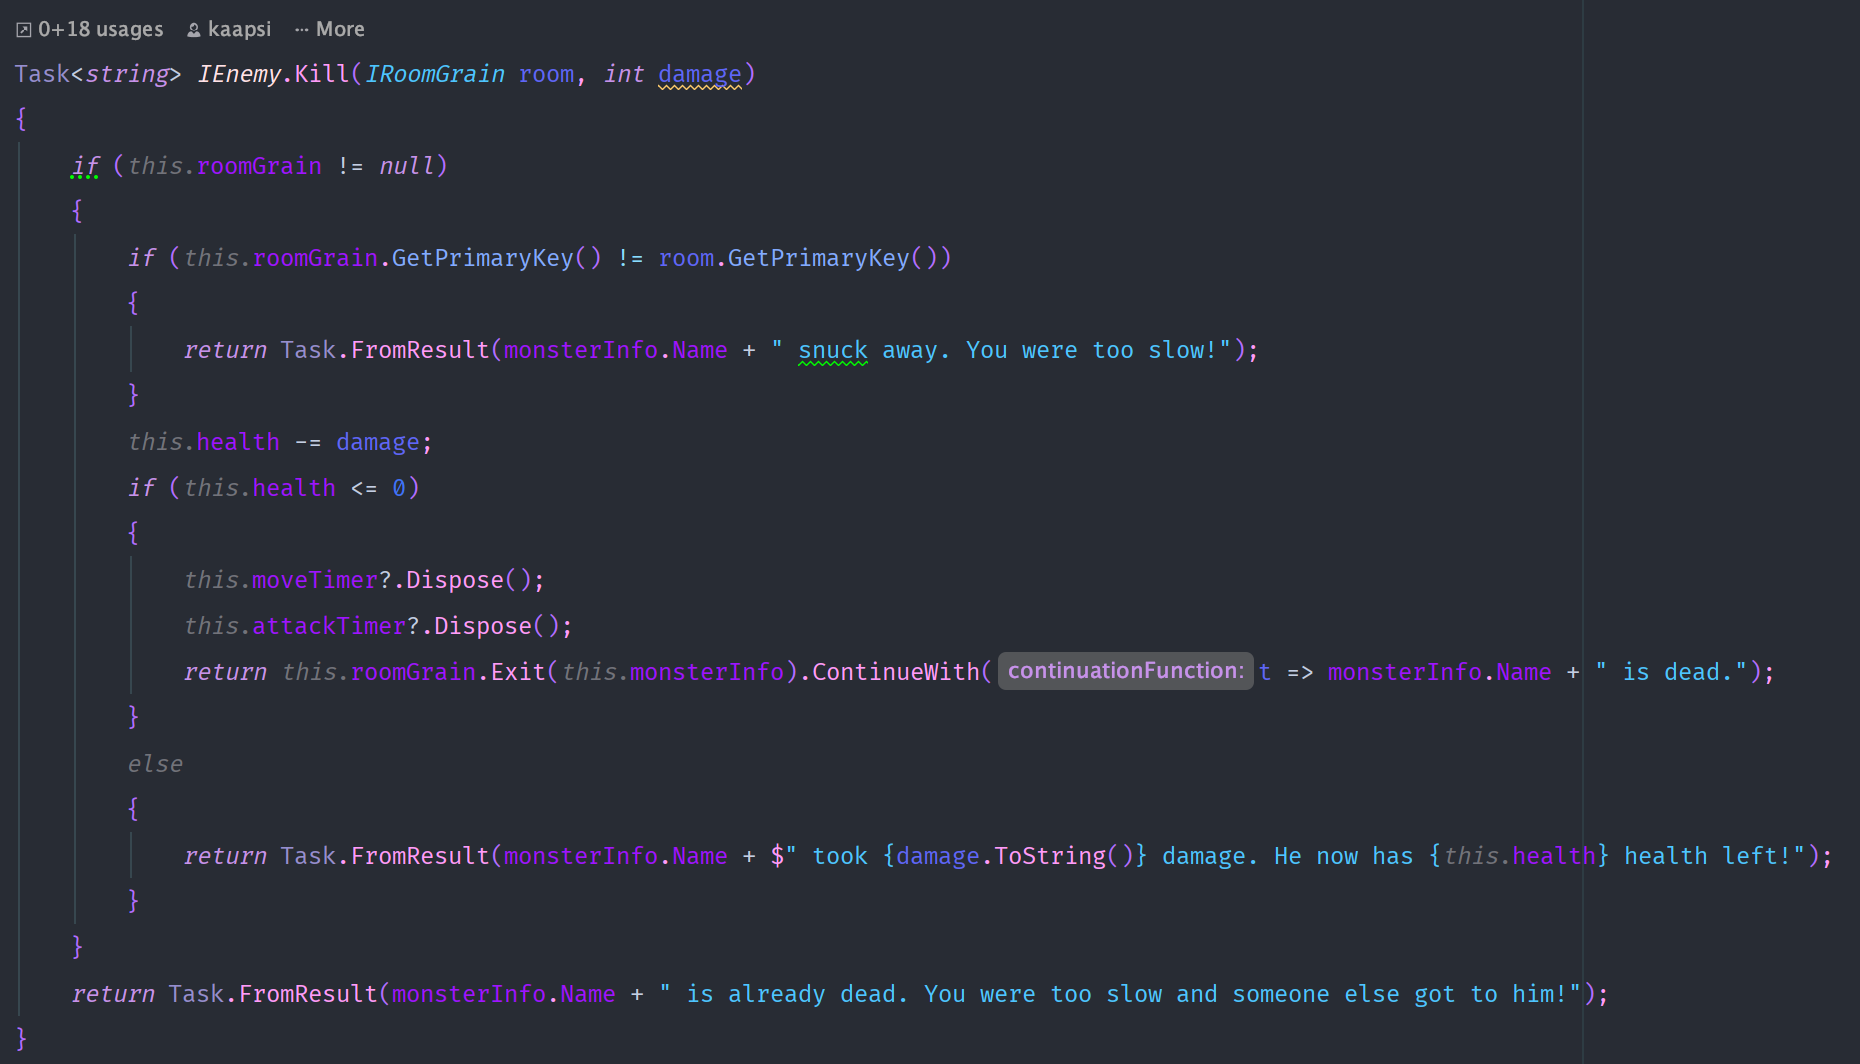
\includegraphics[width=\linewidth]{Materials/Decomposition/Boss/MonsterKill}
	\caption{The monster's method for taking damage.}
	\label{MonsterKill}
\end{figure}

\newpage

\begin{wrapfigure}{R}{0.55\linewidth}
	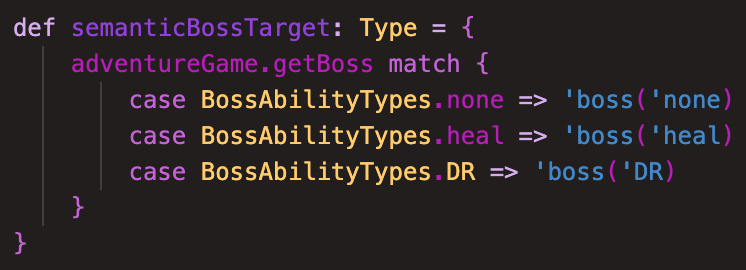
\includegraphics[width=\linewidth]{Materials/Decomposition/Boss/SemanticTarget}
	\caption{Depending on which ability is specified in the metalanguage, we will be looking for different intersections for the boss type.}
	\label{SemanticTargetExample}
\end{wrapfigure}
We found that the boss was a three-part entity, and is defined by its \textit{OnActivateAsync} method, its interaction with the room and perhaps most obviously its ability. We have named the semantic types for each part \textit{'bossOnActivateAsync'}, \textit{'bossRoomInteraction'} and \textit{'bossAbility'} respectively. All the semantic types are intersected by the kinding \textit{'bossAbility'} which can be either \textit{'heal'} or \textit{'DR'} (damage reduction). In our metalanguage we have defined a boss field which can take one of three enum values: \textit{'heal'}, \textit{'DR'} or \textit{'none'}. In \autoref{MetalanguageSetBoss} we see how we can set the boss to have the damage reduction ability in the metalanguage. In our semantic target we match our metalanguage defined boss field with the enum values and get the semantic type \textit{'boss'} intersected by the matching enum type as seen in \autoref{SemanticTargetExample}.
\begin{figure}[H]
	\centering
	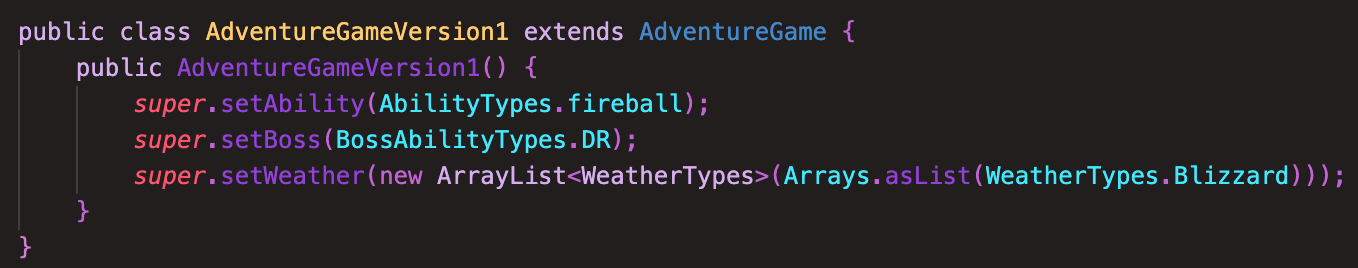
\includegraphics[width=0.95\textwidth]{Materials/Decomposition/Boss/MetalanguageSetBoss}
	\caption{Here we see how the boss is set to have the damage reduction ability in the metalanguage.}
	\label{MetalanguageSetBoss}
\end{figure}

For the semantic type \textit{'bossOnActivateAsync'} we have two combinators, one where the timer for the monster healing ability is started, and one where it is not. Otherwise there is a small additional setup for the boss which is the same for both combinators.\\
The two combinators for the abilities are also very simple. The variation with the heal ability implements the \textit{HealAdds} method whereas the variation with damage reduction is just an empty string. This is because there is no method for the damage reduction, its just a flag which is set whenever the boss spawns a new add.\\
This leaves us with the interaction between the room and the boss. To remove the damage reduction from the boss it needs to know when the adds die. For this we have added an observer like pattern between the room's \textit{Exit} method and the boss. Usually when implementing the observer pattern, several objects wants to know that something has changed in a single object, and so the single object broadcasts that this change has happened rather than the many objects asking \textit{if} there have been a change. Here the room knows when the adds dies, namely when the \textit{Exit} method is called. We thus changed the \textit{Exit} method to call the boss' \textit{UpdateAdds} method. This is obviously dead code in the variations where we do not have any boss, and so we make a check for the boss being present in the room. The semantic type \textit{'bossRoomInteraction'} include the \textit{UpdateAdds} as it is here we set the damage reduction flag back to false, but it also includes the \textit{SpawnAdds} method as it is here we set the flag to true. Given \textit{SpawnAdds} calls the room's \textit{Enter} function (and thus has an interaction with the room) for the newly created monster, we thought it would be fine to include both methods in the same combinator instead of creating more types and more complexity.\\
We here notice somewhat the same issue as with the player's abilities, namely that they do not share the same purpose. We see that the two abilities only changes a single line in \textit{SpawnAdds} and only a few lines in \textit{UpdateAdds} where the damage reduction flag is set. At first, one would think we could use dependency injection to define a common interface for boss abilities. But this would require the statement which sets the damage reduction flag in \textit{SpawnAdds} to be replaced by a call to an ability use, which would execute the healing ability each time an add is spawned which is not what we want. We here notice that the healing ability is on a timer whereas the damage reduction has a more event driven behaviour as it triggers when an add is spawned and when an add is killed, and the 'nature' of the two abilities are thus different. Using dependency injection would require one of the abilities to change 'nature' as either we would need to heal every time an add is spawned, or we would need to provide damage reduction on a timer. Changing the damage reduction to be on a timer which aligns with the timer for \textit{SpawnAdds} could work as it would remove the one-liner from \textit{SpawnAdds}, but we remove the synchronization of the damage reduction and the add spawning, and risk that an attack hits the boss between the add spawn and the damage reduction. We found that our implementation is the best solution to the issue although it to some extent limits the extendability of the boss.\todo{måske noget visualisering?}\\
For the variations with no boss we created a combinator which requires nothing, but creates a semantic type of \textit{'boss} intersected with \textit{'none} where the boss grain is simply empty.\\

One might now ask, how do we spawn the boss? This is done in \textit{'Adventure.cs'} where we add the method \textit{AddBoss}. This of course would also have to be synthesized and so if a boss is set in our metalanguage we have a combinator with our changes added, and if we are having a variation without a boss we have a combinator without our changes. We tried to merge this synthesis with the boss, but due to the limitation of only being able to create one file per job added to the CLS we had to split the synthesis in two.\\

In conclusion we found that the best way to ensure disposal of timers is to make it the only 'path' possible. We did this by only having one way for the monsters and the boss to exit the game, and that involved disposing their timers first. For safety we decided this was best done in unsynthesized code as this would ensure uniform behaviour no matter what variation we create.\\
We also see that spawning additional actors is no problem in a synthesized setting, and this can easily be achieved on a timer as with the boss. The only problem we encounter is created by us, and is how we have weaved the damage reduction ability into the add spawning. Although this approach to us seems better than the alternatives, it still limits the extendability of the boss.
\subsection{Room}
\begin{itemize}
	\item Dependency injection of weather effect objects.
	\item Strategy pattern.
	\item writing 4 kindings, one for each weather
	\item 'abuse' strings and make it dynamic
\end{itemize}

\subsection{Good decomposition}
One can now raise the question, did we achieve good decomposition? To answer that, we would need to look at what makes a good component. This has been a difficult task to answer, as it has been hard to find literature that answers that question. The closest we have got is \cite{Components}, but the focus can be seen to be on a bit higher level than our decomposition. \cite{Components} gives the impression that a component is a collection of code wrapped in a well defined and well documented interface. The focus is on how the component will be communicating with the other classes of the system through its interface, and so there is great emphasis on the design. We can look at this from two angles. We can look at our components as the actors of our system, the player, room, monsters and boss. Here we see encapsulated units with some dependencies on each other and well defined interfaces for the interaction they have with each other. We here have some units which could be reused in another game which is structured the same way. However, we can also look at each of the actors and decompose them. It is here it gets a little uglier and many of the issues described in the previous subsections arise. When we decomposed the actors we did not create a standard for what the components should be and thus we did not create interfaces for them. We have already discussed when it would have made sense and when not to use dependency injection, but not using interfaces makes it hard to reuse components in other projects, and so looking at our individual combinators, its not a lot of them that are reusable. We did not really intend each combinator to be reusable by itself as our goal was to combinate the actors. Our goal was to create interesting variations which were not too similar, and we believe that we succeeded there. However, depending on which angle we look at our decomposition, we get different results. Although less coupling and less dependency on the room would be preferable, we still feel our actors are encapsulated and independent. It is hard to keep both the single responsibility principle and have no coupling, and so we feel we have a good trade off. If we look at the system as a whole, the actors becomes some of the components and although some design decisions have made it hard to extend them we see them as decent components, and thus we have achieved somewhat good decomposition.\\
Had our goal been to create the components for our actors, we would probably not have been combinating our actors as a whole, but instead creating smaller classes like a 'PlayerAbility' class which we would then create different methods for. The end goal would be the same, a player with an ability, but here all the combinators would be reusable. It is thus important to distinguish the two viewpoints from each other when we evaluate our decomposition as they yield two very different results. We can however compare the two approaches, and conclude that we have probably chosen the wrong approach due to both simplicity and the amount of combinators which could be made reusable.

\subsection{Future work}
In future work with the CLS and Orleans we cannot put enough emphasis on how important a good solid design is. When we began learning about the CLS we thought it would eliminate the need for dependency injection, we just replace code so why make a socket for it? After working on this project we now understand the importance and we understand that the CLS does not replace any already existing software engineering principles, on the contrary, using the CLS makes it much more important to follow them. Both the CLS and Orleans strive to work with encapsulated and isolated code which has no to little coupling with other entities, and so they both seem and feel to be a great match together, also for future projects.